

\spis{O~przydziale miejsc na przedmiotach}
{Oskar Skibski}

\wtyt{\hspace*{-5.5cm}O~przydziale miejsc na przedmiotach\hfill
\waut{Oskar SKIBSKI*}}

\aafil{Wydział Matematyki, Informatyki i~Mechaniki, Uniwersytet Warszawski}
Kilka miesięcy temu Samorząd Studentów Wydziału Matematyki, Informatyki i~Mechaniki Uniwersytetu Warszawskiego zaproponował, aby zmienić sposób, w~jaki odbywa się rejestracja studentów na przedmioty.
Do tej pory, w~uproszczeniu, działała ona tak: każdy student wybierał przedmioty, na które chciałby się zapisać; następnie po kolei rozpatrywani byli studenci, w~kolejności malejącej średniej ocen, i~każdemu przydzielane były miejsca na wszystkich przedmiotach, które wybrali i~na które były jeszcze wolne miejsca. 
%W rezultacie osoby z najwyższą średnią dostawały wszystkie co chciały, osoby ze średnią średnią musiały zadowolić się przedmiotami drugiego wyboru, a z niską -- tym co zostało.
Studenci nie byli zbytnio zadowoleni z~tego systemu, i~trudno im się dziwić. Jednym z~problemów było to, że student nie wiedział, ile przedmiotów powinien wybrać, bo nie miał pewności, ile z~nich dostanie, a~ileś zaliczyć musi. Większym problemem było jednak to, że system ten bardzo mocno premiował osoby z~wysoką średnią. 
Można argumentować, że student z~najwyższą średnią powinien mieć pierwszeństwo rejestracji na pewną liczbę przedmiotów przed studentem ze średnią najniższą. 
Ale czy powinien też mieć pierwszeństwo na wszystkich przedmiotach przed studentem ze średnią tylko odrobinę niższą? 
\marg{Podobno zdarzało się nawet, że studenci z~wysoką średnią rejestrowali się na jakiś przedmiot ,,dla kogoś'', a~potem na papierowych druczkach w~Sekcji Studenckiej oddawali mu to miejsce.}

Pierwszym naturalnym krokiem do uzdrowienia systemu było wprowadzenie limitu na liczbę przedmiotów, jakie może dostać jeden student, oraz zmiana tego, co deklarują studenci -- lepiej, aby podawali oni kolejność przedmiotów, na które chcą się zarejestrować, od najbardziej pożądanego do najmniej.
Trudniejszym problemem jest jednak wyrównanie szans studentów.
Najrówniej byłoby oczywiście, gdyby w~kółko każdemu studentowi przydzielać jeden przedmiot. Ten system, znany na przykład z~wyboru drużyn na lekcjach wf, nazywa się \emph{Round Robin} (lub rzadziej, ale po polsku, \emph{algorytmem karuzelowym}).
Jednak czy tak powinna działać rejestracja na przedmioty? Czy ciężko wypracowana średnia nie powinna  odgrywać większej roli? Czy dałoby się zrobić tak, aby osoby ze zbliżoną średnią były traktowane tak równo, jak się da, ale większa różnica w~średnich przekładała się na lepszą sytuację?

\marg{W~dyskusjach i~opracowaniu tej metody uczestniczyło sporo osób: Marcin Engel, Agata Janowska, Piotr Kępczyński, Paulina Kubera, Adam Malinowski, Konrad Mocarski, Jakub~Piotrowicz, Barbara Próchniak, Oskar Skibski i~Piotr~Skowron (kolejność alfabetyczna).}
Pewnie, że się da! W~wyniku wielu rozmów i~negocjacji powstał algorytm, który ze względu na swoją uderzającą sprawiedliwość nazwany został \emph{Robin Hoodem}.

\fbox{\parbox{\textwidth}{
{\color{magenta}\textbf{\underline{Przydział miejsc na przedmiotach \emph{(Robin Hood)}}}}
\begin{description}\vspace*{6pt}
\item[Krok 1:] Każdy student podaje ranking przedmiotów, na jakie chciałby się zapisać.
\item[Krok 2:] Umieszczamy wszystkich studentów na wspólnej liście i~sortujemy malejąco względem średniej ocen.
\item[Krok 3:] Bierzemy pierwszą osobę z~listy i~przydzielamy jej przedmiot, na którym zależy jej najbardziej spośród tych, na których są jeszcze wolne miejsca (jeżeli jeszcze nie osiągnęła pewnego z~góry ustalonego limitu).
\item[Krok 4:] Zmniejszamy średnią wybranej osobie o~stałą $c = 0{,}5$ i~przesuwamy ją odpowiednio w~dół na liście.
\item[Krok 5:] Powtarzamy kroki 3 i~4, aż  skończą się nam miejsca na przedmiotach lub nikt nie będzie chciał już żadnego z~dostępnych przedmiotów.
\end{description}}}

Ile powinna wynosić stała $c,$ jest kwestią do dyskusji.
Łatwo zauważyć, że gdyby zmienić ją na $0$, to uzyskalibyśmy obecny system, a~dla $5$ to zwykły Round Robin.

A~co ta stała oznacza? Ustalmy dwóch studentów i~popatrzmy, jak przeplatają się ich wybory. Jeżeli dwie osoby mają różnicę średnich mniejszą niż $c$, to są traktowane tak równo, jak się da -- będą wybierać na zmianę, zaczynając od tej z~wyższą średnią. Jeżeli z~kolei ta różnica jest pomiędzy $k \cdot c$ a $(k+1) \cdot c$, to student z~wyższą średnią najpierw wybierze $k$ przedmiotów, a~potem będą wybierać na zmianę, zaczynając od tego z~wyższą średnią.
Na przykład dla najwyższej średniej $5{,}0$ i~najniższej $3{,}1$, najlepszy student wybierze 4 przedmioty przed najgorszym.

Możemy się spierać, czy metoda jest fajna, czy nie. W~szanowanym czasopiśmie, jakim jest \emph{Delta}, skupimy się jednak na konkretach, czyli zbadamy, jakie ma teoretyczne własności. Ale najpierw ilustracja.\marg{
\includegraphics{art/202501_kol01}}

\begin{figure}[ht]\hspace*{-5cm}
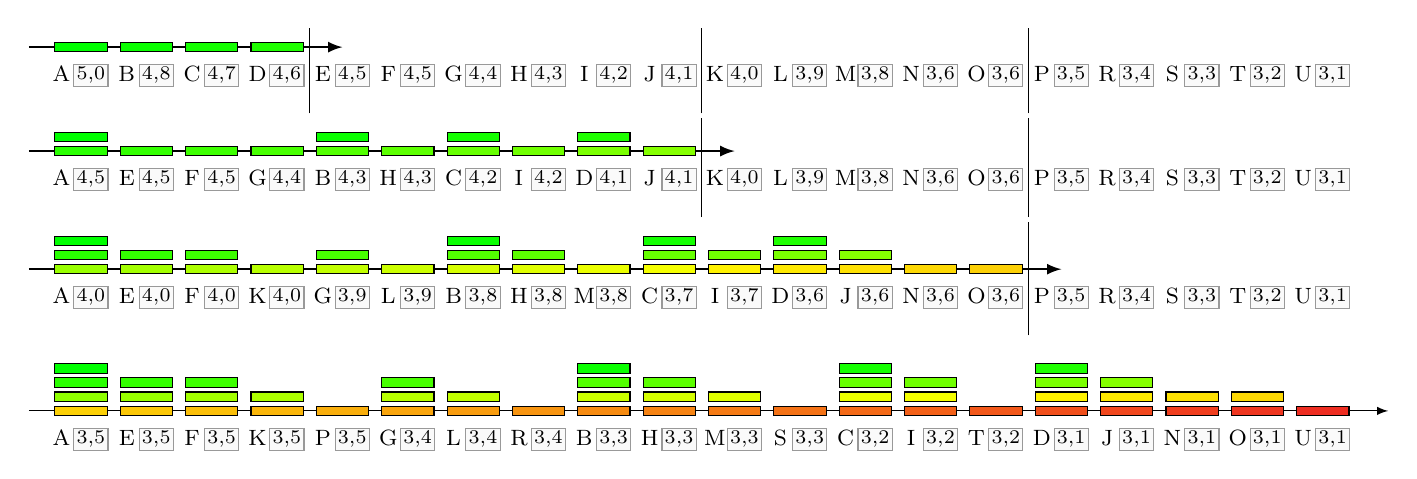
\begin{tikzpicture}[x=0.83cm,y=0.6cm] % change these values to adjust the size of a figure
  \tikzset{     
    e4c node/.style={rectangle,draw=black!40,fill=black!02,minimum size=0.28cm,inner sep=1pt,font={\scriptsize}}, 
    e4c node2/.style={},%rectangle,draw,minimum size=0.10cm,inner sep=0}, 
    e4c nodet/.style={rectangle,draw=none,minimum size=0.28cm,inner sep=1pt,font={\footnotesize}}, 
    node-label/.style={below=4pt}, 
    e4c edge/.style={bend right=30,sloped,above,font=\footnotesize,-latex}
  }

  \def\xt{-0.3};
  \def\yt{0.03};
  
  \def\xn{0.15};
  \def\yn{0.0};

  \def\y{-0.8};
  \draw (4.5,\y-0.8) -- (4.5,\y+1);
  \draw (10.5,\y-0.8) -- (10.5,\y+1);
  \draw (15.5,\y-0.8) -- (15.5,\y+1);
  
  \draw[-latex,thick] (0.2,\y+0.6) -- (5.0,\y+0.6);
 
\node[e4c nodet] at (1+\xt, \y+\yt) {A}; 
\node[e4c nodet] at (2+\xt, \y+\yt) {B}; 
\node[e4c nodet] at (3+\xt, \y+\yt) {C};
\node[e4c nodet] at (4+\xt, \y+\yt) {D};
\node[e4c nodet] at (5+\xt, \y+\yt) {E};
\node[e4c nodet] at (6+\xt, \y+\yt) {F}; 
\node[e4c nodet] at (7+\xt, \y+\yt) {G}; 
\node[e4c nodet] at (8+\xt, \y+\yt) {H};
\node[e4c nodet] at (9+\xt, \y+\yt) {I};
\node[e4c nodet] at (10+\xt, \y+\yt) {J};
\node[e4c nodet] at (11+\xt, \y+\yt) {K}; 
\node[e4c nodet] at (12+\xt, \y+\yt) {L}; 
\node[e4c nodet] at (13+\xt, \y+\yt) {M};
\node[e4c nodet] at (14+\xt, \y+\yt) {N};
\node[e4c nodet] at (15+\xt, \y+\yt) {O};
\node[e4c nodet] at (16+\xt, \y+\yt) {P}; 
\node[e4c nodet] at (17+\xt, \y+\yt) {R}; 
\node[e4c nodet] at (18+\xt, \y+\yt) {S};
\node[e4c nodet] at (19+\xt, \y+\yt) {T};
\node[e4c nodet] at (20+\xt, \y+\yt) {U};

\node[e4c node] (1) at (1+\xn, \y+\yn) {$5{,}0$}; 
\filldraw[fill=green!100!yellow] (1-0.4,\y+0.5) rectangle (1+0.4,\y+0.7); 
\node[e4c node] (2) at (2+\xn, \y+\yn) {$4{,}8$}; 
\filldraw[fill=green!96!yellow] (2-0.4,\y+0.5) rectangle (2+0.4,\y+0.7); 
\node[e4c node] (3) at (3+\xn, \y+\yn) {$4{,}7$}; 
\filldraw[fill=green!92!yellow] (3-0.4,\y+0.5) rectangle (3+0.4,\y+0.7); 
\node[e4c node] (4) at (4+\xn, \y+\yn) {$4{,}6$}; 
\filldraw[fill=green!88!yellow] (4-0.4,\y+0.5) rectangle (4+0.4,\y+0.7); 
\node[e4c node] (5) at (5+\xn, \y+\yn) {$4{,}5$}; 
\node[e4c node] (6) at (6+\xn, \y+\yn) {$4{,}5$}; 
\node[e4c node] (7) at (7+\xn, \y+\yn) {$4{,}4$}; 
\node[e4c node] (8) at (8+\xn, \y+\yn) {$4{,}3$}; 
\node[e4c node] (9) at (9+\xn, \y+\yn) {$4{,}2$}; 
\node[e4c node] (10) at (10+\xn, \y+\yn) {$4{,}1$}; 
\node[e4c node] (11) at (11+\xn, \y+\yn) {$4{,}0$}; 
\node[e4c node] (12) at (12+\xn, \y+\yn) {$3{,}9$}; 
\node[e4c node] (13) at (13+\xn, \y+\yn) {$3{,}8$}; 
\node[e4c node] (14) at (14+\xn, \y+\yn) {$3{,}6$}; 
\node[e4c node] (15) at (15+\xn, \y+\yn) {$3{,}6$}; 
\node[e4c node] (16) at (16+\xn, \y+\yn) {$3{,}5$}; 
\node[e4c node] (17) at (17+\xn, \y+\yn) {$3{,}4$}; 
\node[e4c node] (18) at (18+\xn, \y+\yn) {$3{,}3$}; 
\node[e4c node] (19) at (19+\xn, \y+\yn) {$3{,}2$}; 
\node[e4c node] (20) at (20+\xn, \y+\yn) {$3{,}1$}; 

%%%%%%%%%%%%%%%%%%%%%%%%%%%%%%%%

  \def\y{-3};
  \draw (10.5,\y-0.8) -- (10.5,\y+1.3);
  \draw (15.5,\y-0.8) -- (15.5,\y+1.3);

  \draw[-latex,thick] (0.2,\y+0.6) -- (11.0,\y+0.6);
 
  \node[e4c nodet] at (1+\xt, \y+\yt) {A}; 
  \node[e4c nodet] at (2+\xt, \y+\yt) {E}; 
  \node[e4c nodet] at (3+\xt, \y+\yt) {F};
  \node[e4c nodet] at (4+\xt, \y+\yt) {G};
  \node[e4c nodet] at (5+\xt, \y+\yt) {B};
  \node[e4c nodet] at (6+\xt, \y+\yt) {H}; 
  \node[e4c nodet] at (7+\xt, \y+\yt) {C}; 
  \node[e4c nodet] at (8+\xt, \y+\yt) {I};
  \node[e4c nodet] at (9+\xt, \y+\yt) {D};
  \node[e4c nodet] at (10+\xt, \y+\yt) {J};
  \node[e4c nodet] at (11+\xt, \y+\yt) {K}; 
  \node[e4c nodet] at (12+\xt, \y+\yt) {L}; 
  \node[e4c nodet] at (13+\xt, \y+\yt) {M};
  \node[e4c nodet] at (14+\xt, \y+\yt) {N};
  \node[e4c nodet] at (15+\xt, \y+\yt) {O};
  \node[e4c nodet] at (16+\xt, \y+\yt) {P}; 
  \node[e4c nodet] at (17+\xt, \y+\yt) {R}; 
  \node[e4c nodet] at (18+\xt, \y+\yt) {S};
  \node[e4c nodet] at (19+\xt, \y+\yt) {T};
  \node[e4c nodet] at (20+\xt, \y+\yt) {U};

  \node[e4c node] (1) at (1+\xn, \y+\yn) {$4{,}5$}; 
  \filldraw[fill=green!84!yellow] (1-0.4,\y+0.5) rectangle (1+0.4,\y+0.7); 
  \filldraw[fill=green!100!yellow] (1-0.4,\y+0.8) rectangle (1+0.4,\y+1.0); 
  \node[e4c node] (2) at (2+\xn, \y+\yn) {$4{,}5$}; 
  \filldraw[fill=green!80!yellow] (2-0.4,\y+0.5) rectangle (2+0.4,\y+0.7); 
  \node[e4c node] (3) at (3+\xn, \y+\yn) {$4{,}5$}; 
  \filldraw[fill=green!76!yellow] (3-0.4,\y+0.5) rectangle (3+0.4,\y+0.7); 
  \node[e4c node] (4) at (4+\xn, \y+\yn) {$4{,}4$}; 
  \filldraw[fill=green!72!yellow] (4-0.4,\y+0.5) rectangle (4+0.4,\y+0.7); 
  \node[e4c node] (5) at (5+\xn, \y+\yn) {$4{,}3$}; 
  \filldraw[fill=green!68!yellow] (5-0.4,\y+0.5) rectangle (5+0.4,\y+0.7); 
  \filldraw[fill=green!96!yellow] (5-0.4,\y+0.8) rectangle (5+0.4,\y+1.0); 
  \node[e4c node] (6) at (6+\xn, \y+\yn) {$4{,}3$}; 
  \filldraw[fill=green!64!yellow] (6-0.4,\y+0.5) rectangle (6+0.4,\y+0.7); 
  \node[e4c node] (7) at (7+\xn, \y+\yn) {$4{,}2$}; 
  \filldraw[fill=green!60!yellow] (7-0.4,\y+0.5) rectangle (7+0.4,\y+0.7); 
  \filldraw[fill=green!92!yellow] (7-0.4,\y+0.8) rectangle (7+0.4,\y+1.0); 
  \node[e4c node] (8) at (8+\xn, \y+\yn) {$4{,}2$}; 
  \filldraw[fill=green!56!yellow] (8-0.4,\y+0.5) rectangle (8+0.4,\y+0.7); 
  \node[e4c node] (9) at (9+\xn, \y+\yn) {$4{,}1$}; 
  \filldraw[fill=green!52!yellow] (9-0.4,\y+0.5) rectangle (9+0.4,\y+0.7); 
  \filldraw[fill=green!88!yellow] (9-0.4,\y+0.8) rectangle (9+0.4,\y+1.0); 
  \node[e4c node] (10) at (10+\xn, \y+\yn) {$4{,}1$}; 
  \filldraw[fill=green!48!yellow] (10-0.4,\y+0.5) rectangle (10+0.4,\y+0.7); 
  \node[e4c node] (11) at (11+\xn, \y+\yn) {$4{,}0$}; 
  \node[e4c node] (12) at (12+\xn, \y+\yn) {$3{,}9$}; 
  \node[e4c node] (13) at (13+\xn, \y+\yn) {$3{,}8$}; 
  \node[e4c node] (14) at (14+\xn, \y+\yn) {$3{,}6$}; 
  \node[e4c node] (15) at (15+\xn, \y+\yn) {$3{,}6$}; 
  \node[e4c node] (16) at (16+\xn, \y+\yn) {$3{,}5$}; 
  \node[e4c node] (17) at (17+\xn, \y+\yn) {$3{,}4$}; 
  \node[e4c node] (18) at (18+\xn, \y+\yn) {$3{,}3$}; 
  \node[e4c node] (19) at (19+\xn, \y+\yn) {$3{,}2$}; 
  \node[e4c node] (20) at (20+\xn, \y+\yn) {$3{,}1$}; 

%%%%%%%%%%%%%%%%%%%%%%%%%%%%%%%%

  \def\y{-5.5};
  \draw (15.5,\y-0.8) -- (15.5,\y+1.6);

  \draw[-latex,thick] (0.2,\y+0.6) -- (16.0,\y+0.6);
 
  \node[e4c nodet] at (1+\xt, \y+\yt) {A}; 
  \node[e4c nodet] at (2+\xt, \y+\yt) {E}; 
  \node[e4c nodet] at (3+\xt, \y+\yt) {F};
  \node[e4c nodet] at (4+\xt, \y+\yt) {K};
  \node[e4c nodet] at (5+\xt, \y+\yt) {G};
  \node[e4c nodet] at (6+\xt, \y+\yt) {L}; 
  \node[e4c nodet] at (7+\xt, \y+\yt) {B}; 
  \node[e4c nodet] at (8+\xt, \y+\yt) {H};
  \node[e4c nodet] at (9+\xt, \y+\yt) {M};
  \node[e4c nodet] at (10+\xt, \y+\yt) {C};
  \node[e4c nodet] at (11+\xt, \y+\yt) {I}; 
  \node[e4c nodet] at (12+\xt, \y+\yt) {D}; 
  \node[e4c nodet] at (13+\xt, \y+\yt) {J};
  \node[e4c nodet] at (14+\xt, \y+\yt) {N};
  \node[e4c nodet] at (15+\xt, \y+\yt) {O};
  \node[e4c nodet] at (16+\xt, \y+\yt) {P}; 
  \node[e4c nodet] at (17+\xt, \y+\yt) {R}; 
  \node[e4c nodet] at (18+\xt, \y+\yt) {S};
  \node[e4c nodet] at (19+\xt, \y+\yt) {T};
  \node[e4c nodet] at (20+\xt, \y+\yt) {U};

  \node[e4c node] (1) at (1+\xn, \y+\yn) {$4{,}0$}; %3
  \filldraw[fill=green!40!yellow] (1-0.4,\y+0.5) rectangle (1+0.4,\y+0.7); 
  \filldraw[fill=green!84!yellow] (1-0.4,\y+0.8) rectangle (1+0.4,\y+1.0); 
  \filldraw[fill=green!100!yellow] (1-0.4,\y+1.1) rectangle (1+0.4,\y+1.3); 
  \node[e4c node] (2) at (2+\xn, \y+\yn) {$4{,}0$}; %2 
  \filldraw[fill=green!36!yellow] (2-0.4,\y+0.5) rectangle (2+0.4,\y+0.7); 
  \filldraw[fill=green!80!yellow] (2-0.4,\y+0.8) rectangle (2+0.4,\y+1.0); 
  \node[e4c node] (3) at (3+\xn, \y+\yn) {$4{,}0$}; %2
  \filldraw[fill=green!32!yellow] (3-0.4,\y+0.5) rectangle (3+0.4,\y+0.7); 
  \filldraw[fill=green!76!yellow] (3-0.4,\y+0.8) rectangle (3+0.4,\y+1.0); 
  \node[e4c node] (4) at (4+\xn, \y+\yn) {$4{,}0$}; %1 
  \filldraw[fill=green!28!yellow] (4-0.4,\y+0.5) rectangle (4+0.4,\y+0.7); 
  \node[e4c node] (5) at (5+\xn, \y+\yn) {$3{,}9$}; %2
  \filldraw[fill=green!24!yellow] (5-0.4,\y+0.5) rectangle (5+0.4,\y+0.7); 
  \filldraw[fill=green!72!yellow] (5-0.4,\y+0.8) rectangle (5+0.4,\y+1.0); 
  \node[e4c node] (6) at (6+\xn, \y+\yn) {$3{,}9$}; %1
  \filldraw[fill=green!20!yellow] (6-0.4,\y+0.5) rectangle (6+0.4,\y+0.7); 
  \node[e4c node] (7) at (7+\xn, \y+\yn) {$3{,}8$}; %3
  \filldraw[fill=green!16!yellow] (7-0.4,\y+0.5) rectangle (7+0.4,\y+0.7); 
  \filldraw[fill=green!68!yellow] (7-0.4,\y+0.8) rectangle (7+0.4,\y+1.0); 
  \filldraw[fill=green!96!yellow] (7-0.4,\y+1.1) rectangle (7+0.4,\y+1.3); 
  \node[e4c node] (8) at (8+\xn, \y+\yn) {$3{,}8$}; %2 
  \filldraw[fill=green!12!yellow] (8-0.4,\y+0.5) rectangle (8+0.4,\y+0.7); 
  \filldraw[fill=green!64!yellow] (8-0.4,\y+0.8) rectangle (8+0.4,\y+1.0); 
  \node[e4c node] (9) at (9+\xn, \y+\yn) {$3{,}8$}; %1
  \filldraw[fill=green!08!yellow] (9-0.4,\y+0.5) rectangle (9+0.4,\y+0.7); 
  \node[e4c node] (10) at (10+\xn, \y+\yn) {$3{,}7$}; %3 
  \filldraw[fill=green!04!yellow] (10-0.4,\y+0.5) rectangle (10+0.4,\y+0.7); 
  \filldraw[fill=green!60!yellow] (10-0.4,\y+0.8) rectangle (10+0.4,\y+1.0); 
  \filldraw[fill=green!92!yellow] (10-0.4,\y+1.1) rectangle (10+0.4,\y+1.3); 
  \node[e4c node] (11) at (11+\xn, \y+\yn) {$3{,}7$}; %2 
  \filldraw[fill=green!00!yellow] (11-0.4,\y+0.5) rectangle (11+0.4,\y+0.7); 
  \filldraw[fill=green!56!yellow] (11-0.4,\y+0.8) rectangle (11+0.4,\y+1.0); 
  \node[e4c node] (12) at (12+\xn, \y+\yn) {$3{,}6$}; %3
  \filldraw[fill=yellow!96!red] (12-0.4,\y+0.5) rectangle (12+0.4,\y+0.7); 
  \filldraw[fill=green!52!yellow] (12-0.4,\y+0.8) rectangle (12+0.4,\y+1.0); 
  \filldraw[fill=green!88!yellow] (12-0.4,\y+1.1) rectangle (12+0.4,\y+1.3); 
  \node[e4c node] (13) at (13+\xn, \y+\yn) {$3{,}6$}; %2
  \filldraw[fill=yellow!92!red] (13-0.4,\y+0.5) rectangle (13+0.4,\y+0.7); 
  \filldraw[fill=green!48!yellow] (13-0.4,\y+0.8) rectangle (13+0.4,\y+1.0); 
  \node[e4c node] (14) at (14+\xn, \y+\yn) {$3{,}6$}; %1
  \filldraw[fill=yellow!88!red] (14-0.4,\y+0.5) rectangle (14+0.4,\y+0.7); 
  \node[e4c node] (15) at (15+\xn, \y+\yn) {$3{,}6$}; %1
  \filldraw[fill=yellow!84!red] (15-0.4,\y+0.5) rectangle (15+0.4,\y+0.7); 
  \node[e4c node] (16) at (16+\xn, \y+\yn) {$3{,}5$}; 
  \node[e4c node] (17) at (17+\xn, \y+\yn) {$3{,}4$}; 
  \node[e4c node] (18) at (18+\xn, \y+\yn) {$3{,}3$}; 
  \node[e4c node] (19) at (19+\xn, \y+\yn) {$3{,}2$}; 
  \node[e4c node] (20) at (20+\xn, \y+\yn) {$3{,}1$}; 

%%%%%%%%%%%%%%%%%%%%%%%%%%%%%%%%

  \def\y{-8.5};
 
  \draw[-latex,thin] (0.2,\y+0.6) -- (21.0,\y+0.6);
 
  \node[e4c nodet] at (1+\xt, \y+\yt) {A}; 
  \node[e4c nodet] at (2+\xt, \y+\yt) {E}; 
  \node[e4c nodet] at (3+\xt, \y+\yt) {F};
  \node[e4c nodet] at (4+\xt, \y+\yt) {K};
  \node[e4c nodet] at (5+\xt, \y+\yt) {P};
  \node[e4c nodet] at (6+\xt, \y+\yt) {G};
  \node[e4c nodet] at (7+\xt, \y+\yt) {L}; 
  \node[e4c nodet] at (8+\xt, \y+\yt) {R}; 
  \node[e4c nodet] at (9+\xt, \y+\yt) {B}; 
  \node[e4c nodet] at (10+\xt, \y+\yt) {H};
  \node[e4c nodet] at (11+\xt, \y+\yt) {M};
  \node[e4c nodet] at (12+\xt, \y+\yt) {S};
  \node[e4c nodet] at (13+\xt, \y+\yt) {C};
  \node[e4c nodet] at (14+\xt, \y+\yt) {I}; 
  \node[e4c nodet] at (15+\xt, \y+\yt) {T};
  \node[e4c nodet] at (16+\xt, \y+\yt) {D}; 
  \node[e4c nodet] at (17+\xt, \y+\yt) {J};
  \node[e4c nodet] at (18+\xt, \y+\yt) {N};
  \node[e4c nodet] at (19+\xt, \y+\yt) {O};
  \node[e4c nodet] at (20+\xt, \y+\yt) {U};

  \node[e4c node] (1) at (1+\xn, \y+\yn) {$3{,}5$};
  \filldraw[fill=yellow!84!red] (1-0.4,\y+0.5) rectangle (1+0.4,\y+0.7); 
  \filldraw[fill=green!44!yellow] (1-0.4,\y+0.8) rectangle (1+0.4,\y+1.0); 
  \filldraw[fill=green!84!yellow] (1-0.4,\y+1.1) rectangle (1+0.4,\y+1.3); 
  \filldraw[fill=green!100!yellow] (1-0.4,\y+1.4) rectangle (1+0.4,\y+1.6); 
  \node[e4c node] (2) at (2+\xn, \y+\yn) {$3{,}5$};
  \filldraw[fill=yellow!80!red] (2-0.4,\y+0.5) rectangle (2+0.4,\y+0.7); 
  \filldraw[fill=green!40!yellow] (2-0.4,\y+0.8) rectangle (2+0.4,\y+1.0); 
  \filldraw[fill=green!80!yellow] (2-0.4,\y+1.1) rectangle (2+0.4,\y+1.3); 
  \node[e4c node] (3) at (3+\xn, \y+\yn) {$3{,}5$};
  \filldraw[fill=yellow!76!red] (3-0.4,\y+0.5) rectangle (3+0.4,\y+0.7); 
  \filldraw[fill=green!36!yellow] (3-0.4,\y+0.8) rectangle (3+0.4,\y+1.0); 
  \filldraw[fill=green!76!yellow] (3-0.4,\y+1.1) rectangle (3+0.4,\y+1.3); 
  \node[e4c node] (4) at (4+\xn, \y+\yn) {$3{,}5$};
  \filldraw[fill=yellow!72!red] (4-0.4,\y+0.5) rectangle (4+0.4,\y+0.7); 
  \filldraw[fill=green!32!yellow] (4-0.4,\y+0.8) rectangle (4+0.4,\y+1.0); 
  \node[e4c node] (5) at (5+\xn, \y+\yn) {$3{,}5$};
  \filldraw[fill=yellow!68!red] (5-0.4,\y+0.5) rectangle (5+0.4,\y+0.7); 
  \node[e4c node] (6) at (6+\xn, \y+\yn) {$3{,}4$};
  \filldraw[fill=yellow!64!red] (6-0.4,\y+0.5) rectangle (6+0.4,\y+0.7); 
  \filldraw[fill=green!28!yellow] (6-0.4,\y+0.8) rectangle (6+0.4,\y+1.0); 
  \filldraw[fill=green!72!yellow] (6-0.4,\y+1.1) rectangle (6+0.4,\y+1.3); 
  \node[e4c node] (7) at (7+\xn, \y+\yn) {$3{,}4$};
  \filldraw[fill=yellow!60!red] (7-0.4,\y+0.5) rectangle (7+0.4,\y+0.7); 
  \filldraw[fill=green!24!yellow] (7-0.4,\y+0.8) rectangle (7+0.4,\y+1.0); 
  \node[e4c node] (8) at (8+\xn, \y+\yn) {$3{,}4$};
  \filldraw[fill=yellow!56!red] (8-0.4,\y+0.5) rectangle (8+0.4,\y+0.7); 
  \node[e4c node] (9) at (9+\xn, \y+\yn) {$3{,}3$};
  \filldraw[fill=yellow!52!red] (9-0.4,\y+0.5) rectangle (9+0.4,\y+0.7); 
  \filldraw[fill=green!20!yellow] (9-0.4,\y+0.8) rectangle (9+0.4,\y+1.0); 
  \filldraw[fill=green!68!yellow] (9-0.4,\y+1.1) rectangle (9+0.4,\y+1.3); 
  \filldraw[fill=green!96!yellow] (9-0.4,\y+1.4) rectangle (9+0.4,\y+1.6); 
  \node[e4c node] (10) at (10+\xn, \y+\yn) {$3{,}3$};
  \filldraw[fill=yellow!48!red] (10-0.4,\y+0.5) rectangle (10+0.4,\y+0.7); 
  \filldraw[fill=green!16!yellow] (10-0.4,\y+0.8) rectangle (10+0.4,\y+1.0); 
  \filldraw[fill=green!64!yellow] (10-0.4,\y+1.1) rectangle (10+0.4,\y+1.3); 
  \node[e4c node] (11) at (11+\xn, \y+\yn) {$3{,}3$};
  \filldraw[fill=yellow!44!red] (11-0.4,\y+0.5) rectangle (11+0.4,\y+0.7); 
  \filldraw[fill=green!12!yellow] (11-0.4,\y+0.8) rectangle (11+0.4,\y+1.0); 
  \node[e4c node] (12) at (12+\xn, \y+\yn) {$3{,}3$};
  \filldraw[fill=yellow!40!red] (12-0.4,\y+0.5) rectangle (12+0.4,\y+0.7); 
  \node[e4c node] (13) at (13+\xn, \y+\yn) {$3{,}2$};
  \filldraw[fill=yellow!36!red] (13-0.4,\y+0.5) rectangle (13+0.4,\y+0.7); 
  \filldraw[fill=green!08!yellow] (13-0.4,\y+0.8) rectangle (13+0.4,\y+1.0); 
  \filldraw[fill=green!60!yellow] (13-0.4,\y+1.1) rectangle (13+0.4,\y+1.3); 
  \filldraw[fill=green!92!yellow] (13-0.4,\y+1.4) rectangle (13+0.4,\y+1.6); 
  \node[e4c node] (14) at (14+\xn, \y+\yn) {$3{,}2$};
  \filldraw[fill=yellow!32!red] (14-0.4,\y+0.5) rectangle (14+0.4,\y+0.7); 
  \filldraw[fill=green!04!yellow] (14-0.4,\y+0.8) rectangle (14+0.4,\y+1.0); 
  \filldraw[fill=green!56!yellow] (14-0.4,\y+1.1) rectangle (14+0.4,\y+1.3); 
  \node[e4c node] (15) at (15+\xn, \y+\yn) {$3{,}2$};
  \filldraw[fill=yellow!28!red] (15-0.4,\y+0.5) rectangle (15+0.4,\y+0.7); 
  \node[e4c node] (16) at (16+\xn, \y+\yn) {$3{,}1$}; 
  \filldraw[fill=yellow!24!red] (16-0.4,\y+0.5) rectangle (16+0.4,\y+0.7); 
  \filldraw[fill=green!00!yellow] (16-0.4,\y+0.8) rectangle (16+0.4,\y+1.0); 
  \filldraw[fill=green!52!yellow] (16-0.4,\y+1.1) rectangle (16+0.4,\y+1.3); 
  \filldraw[fill=green!88!yellow] (16-0.4,\y+1.4) rectangle (16+0.4,\y+1.6); 
  \node[e4c node] (17) at (17+\xn, \y+\yn) {$3{,}1$}; 
  \filldraw[fill=yellow!20!red] (17-0.4,\y+0.5) rectangle (17+0.4,\y+0.7); 
  \filldraw[fill=yellow!96!red] (17-0.4,\y+0.8) rectangle (17+0.4,\y+1.0); 
  \filldraw[fill=green!48!yellow] (17-0.4,\y+1.1) rectangle (17+0.4,\y+1.3); 
  \node[e4c node] (18) at (18+\xn, \y+\yn) {$3{,}1$}; 
  \filldraw[fill=yellow!16!red] (18-0.4,\y+0.5) rectangle (18+0.4,\y+0.7); 
  \filldraw[fill=yellow!92!red] (18-0.4,\y+0.8) rectangle (18+0.4,\y+1.0); 
  \node[e4c node] (19) at (19+\xn, \y+\yn) {$3{,}1$}; 
  \filldraw[fill=yellow!12!red] (19-0.4,\y+0.5) rectangle (19+0.4,\y+0.7); 
  \filldraw[fill=yellow!88!red] (19-0.4,\y+0.8) rectangle (19+0.4,\y+1.0); 
  \node[e4c node] (20) at (20+\xn, \y+\yn) {$3{,}1$}; 
  \filldraw[fill=yellow!08!red] (20-0.4,\y+0.5) rectangle (20+0.4,\y+0.7); 

\end{tikzpicture}
\end{figure}

Ilustracja prezentuje kolejność wyborów w~Robin Hoodzie, a~kolejne wiersze odpowiadają przydziałowi miejsc na przedmiotach po 4, 14, 29 i~49 krokach procedury.
Kolorowe prostokąty symbolizują przydzielane  miejsca, a~kolor odpowiada kolejności, w~której miejsce zostało przyznane -- pierwsze miejsca są zielone, a~ostatnie czerwone.
Jak widzimy, studenci z~najwyższą średnią ($>4{,}5$) wybierają po pierwszym przedmiocie, po czym zmniejszamy im średnią o $0{,}5$. W~ten sposób ,,wtasowują się'' oni w~studentów ze średnią pomiędzy $4{,}0$ a $4{,}5$, i~razem z~nimi wybierają po kolejnym przedmiocie.
   
Aby opowiedzieć o~własnościach Robin Hooda, wprowadźmy trochę oznaczeń. 
Załóżmy, że mamy $n$ ponumerowanych studentów.
Przyjmiemy, że każdy student  ma listę rankingową wszystkich przedmiotów, bez remisów. Dla dwóch przedmiotów $a,b$ będziemy pisać $a \succ_i b,$ jeżeli student $i$ woli przedmiot $a$ od $b$. 
Dla uproszczenia zignorujemy limit przedmiotów, jaki może mieć jeden student: nie zmienia on wiele, a~komplikuje analizę. Będziemy więc każdemu studentowi przydzielać jak najwięcej miejsc.

Między studentów będziemy rozdzielać pewien zbiór miejsc na przedmiotach.
Dla ułatwienia ten zbiór będzie po prostu multizbiorem przedmiotów, czyli ,,zbiorem'', w~którym przedmiot pojawia się tyle razy, ile jest na nim miejsc.
\marg{Przykładowo dla dwóch przedmiotów $m,p$ (matematyka i~polski) możemy mieć multizbiór $O=\{m,m,m,p,p\}$ oznaczający 3 miejsca na matematyce i~2~na~polskim.}
Szukamy pewnego \emph{podziału} tych miejsc, czyli listy $(A_i) = (A_1, \dots, A_n)$ takiej, że $A_1, \dots, A_n$ są zbiorami przedmiotów dla studentów $1,\dots,n$ (nie multizbiorami!), które połączone dadzą multizbiór wszystkich miejsc.

\looseness-1 {\spaceskip.33em minus.1emCo możemy powiedzieć o~preferencjach studenta dla zbiorów przedmiotów?
Aby uniknąć spekulacji, czy lepiej mieć dwa średnie przedmioty, czy jeden fajny i~jeden słaby, będziemy porównywać tylko niektóre zbiory.
Powiemy, że osobie $i$ podoba się zbiór $A$ co najmniej tak samo jak $B$ (oznaczane $A \succeq_i B$), jeżeli $|A| \ge |B|$ oraz najbardziej lubiany przedmiot z $A$ jest co najmniej tak lubiany jak ulubiony z $B$, drugi z $A$ co najmniej tak lubiany jak drugi z $B$ itd.
\marg{Formalnie, $A \succeq_i B,$ jeżeli $|A| \ge |B|$ i~możemy tak uporządkować przedmioty $A = \{a_1, \dots, a_h\}$ i $B = \{b_1, \dots, b_{\ell}\}$, aby zachodziło $a_j=b_j$ lub $a_j \succ_i b_j$ dla każdego $j \in \{1,\dots,{\ell}\}$.} 
Łatwo zauważyć, że $A \succeq_i B$ oraz $B \succeq_i A$ implikuje $A = B$.
Będziemy więc pisać $A \succ_i B,$ jeżeli $A \succeq_i B$ i $A \neq B$.}

Jedną z~podstawowych własności dobrego podziału jest to, że nie da się go łatwo poprawić, to znaczy tak pozmieniać, aby nikt na tym nie stracił, a~ktoś zyskał.

{\leftskip1cm 
Podział $(A_i)$ jest \emph{\color{magenta} optymalny w~sensie Pareto}, jeżeli nie istnieje podział $(B_i)$ taki, że $B_i \succeq_i A_i$ dla każdego studenta $i$ oraz $B_i \succ_i A_i$ dla przynajmniej jednego studenta.
\par}

\looseness-1 Czy podział uzyskany przez Robin Hooda jest w~tym sensie optymalny? Tak. Można powiedzieć nawet więcej -- dowolny podział uzyskany przez kolejne przydzielanie studentom miejsc na ich ulubionych dostępnych przedmiotach jest optymalny, niezależnie od kolejności, w~jakiej będzie się te osoby wybierać.
Aby to zobaczyć, wystarczy po kolei rozpatrywać przyznane miejsca. Czy student  wybierający jako pierwszy może preferować podział, w~którym nie ma przedmiotu, który dostał w~pierwszej kolejce? Oczywiście nie. A~spośród takich podziałów, czy student, który wybiera jako drugi, może preferować podział bez przedmiotu, który dostał w~drugiej kolejce? Nie -- jeżeli nie jest to jego ulubiony przedmiot, to znaczy, że na ulubionym było tylko jedno miejsce, którego nie może dostać, nie krzywdząc w~ten sposób pierwszego studenta. I~tak dalej. 

Nazwijmy taki algorytm przydziału Drunk Robinem
\marg{{\color{magenta}Drunk Robin:} Wybieramy dowolnego studenta i~przydzielamy mu jego ulubiony dostępny przedmiot. Powtarzamy, dopóki są jeszcze jakieś miejsca.}
(definicja na marginesie).
Okazuje się, że wszystkie optymalne podziały da się nim uzyskać! 

\begin{theorem*}
Podział jest optymalny w~sensie Pareto wtedy i~tylko wtedy, gdy da się go uzyskać algorytmem Drunk Robin.
\end{theorem*}
\begin{proof}
Uzasadniliśmy już, że Drunk Robin daje tylko podziały optymalne. Załóżmy, że mamy podział optymalny i~rozpatrzmy graf, w~którym wierzchołkami są studenci, a~skierowana krawędź $(i,j)$ istnieje, jeżeli $j$ posiada jakiś przedmiot, który $i$ woli od wszystkich swoich przedmiotów.
Gdyby ten graf miał cykl, to podział nie byłby optymalny -- każdy student mógłby dostać bardziej lubiany przedmiot w~zamian za któryś mniej lubiany. 
\marg{Jeżeli w~grafie wszystkie wierzchołki mają krawędzie wychodzące, to zawsze znajdziemy w~nim cykl, podążając uparcie za strzałkami wychodzącymi -- studentów (na świecie) mamy skończoną liczbę, więc w~końcu ktoś się powtórzy.}
Skoro graf nie ma cyklu, to musi istnieć wierzchołek bez krawędzi wychodzących, czyli który nikomu nie zazdrości żadnego przedmiotu.
Możemy mu zatem pozwolić wybierać jako pierwszemu. Następnie kasując jego ulubiony przedmiot z~jego zbioru oraz jedno miejsce ze zbioru dostępnych miejsc, dostaniemy mniejszy podział, który też jest optymalny: gdyby nie był i~istniałby lepszy podział, po dodaniu skasowanego przedmiotu dostalibyśmy podział lepszy niż oryginalny, przecząc jego optymalności.
Postępując dla niego i~kolejnych mniejszych podziałów analogicznie, otrzymamy kolejność, w~której każdy student wybiera ulubiony dostępny przedmiot.
\end{proof}

Podziały uzyskane z~Drunk Robina mogą być jednak bardzo niesprawiedliwe. 
W~jaki sposób możemy opisać fakt, że podział jest sprawiedliwy? Nie możemy wymagać, aby wszyscy dostali miejsce na ulubionym przedmiocie. Moglibyśmy jednak chcieć, aby każda osoba miała zbiór nie więcej niż o~jeden przedmiot gorszy niż każda inna.
O~tym właśnie mówi następująca właściwość:

{\leftskip1cm 
Podział $(A_i)$ jest \emph{\color{magenta} wolny od zazdrości z~dokładnością do jednego przedmiotu (EF1),} jeżeli dla dowolnych dwóch studentów $i,j$ zachodzi $A_j = \emptyset$ albo istnieje przedmiot $p \in A_j$, taki że $A_i \succeq_i A_j \setminus \{p\}$.\par}

\marg{{\color{magenta} Round Robin:} Układamy studentów w~listę. Bierzemy pierwszego, przydzielamy mu jego ulubiony dostępny przedmiot i~przesuwamy go na koniec listy. Powtarzamy, dopóki są jeszcze jakieś miejsca.}
Łatwo zobaczyć, że podziały uzyskane Round Robinem spełniają tę własność: 
pierwszy przedmiot wybrany przez studenta $i$ jest dla niego lepszy lub taki sam jak drugi wybrany przez studenta $j$, drugi wybrany przez $i$ jest lepszy lub taki sam jak trzeci wybrany przez $j$ itd.
\marg{Rozważmy 2 studentów, zbiór miejsc $\{a,b,c,d\}$ (na każdym przedmiocie jedno miejsce), podział $A_1 = \{a,b\}$, $A_2 = \{c,d\}$ i~preferencje:
$a \succ_1 b \succ_1 c \succ_1 d$ oraz
$b \succ_2 c \succ_2 d \succ_2 a$.
Podział ten jest optymalny w~sensie Pareto i~spełnia EF1, ale nie da się go uzyskać algorytmem Round Robin.}
Co ciekawe, istnieją jednak podziały optymalne w~sensie Pareto, które spełniają EF1, a~nie da się ich uzyskać algorytmem Round Robin. 
Przykład znajduje się na marginesie.

A~czy podziały uzyskane Robin Hoodem spełniają EF1? 
Nie, ale to dobrze~-- chcemy przecież, aby wyższa średnia przełożyła się na znacząco lepszy zbiór przedmiotów.
Niech $p_i$ będzie pewnym priorytetem, czyli u~nas średnią studenta~$i$.
\marg{Dla modelu, w~którym nie ma limitu przedmiotów, jakie może mieć jeden student, definicja Robin Hooda wygląda tak:\vspace{0.1cm}\newline {\color{magenta} Robin Hood:} Wybieramy studenta z~najwyższą średnią, przydzielamy mu jego ulubiony dostępny przedmiot i~zmniejszamy mu średnią o $c=0{,}5$. Powtarzamy, dopóki są jeszcze jakieś miejsca.}
Możemy zdefiniować następujący wariant własności EF1:

{\leftskip1cm 
Podział $(A_i)$ jest \emph{\color{magenta} wolny od zazdrości z~dokładnością do jednego przedmiotu, uwzględniając priorytety (EF1-$p$),} jeżeli dla dowolnych dwóch studentów $i,j$ zachodzi:
\begin{itemize}[parsep=0pt,topsep=0pt,itemsep=0pt,partopsep=0pt,leftmargin=40pt]
\item jeżeli $(p_j-p_i)/c \in [\ell,\ell+1)$ dla $\ell \in \mathbb{N}$, to istnieje $P \subseteq A_j$, $|P| \le \ell+1$ taki, że $A_i \succeq_i A_j \setminus P,$
\item jeżeli $(p_j-p_i)/c \in (\ell,\ell+1]$ dla $\ell \in \mathbb{N}$, to
istnieje $P \subseteq A_j$, $|P| \le \ell$ taki, że $A_j \setminus P \succeq_j A_i$.
\end{itemize}
\par}

Łatwo sprawdzić, że gdy priorytety są równe, własność ta sprowadza się do EF1.
Przy priorytetach spełnialność wynika z~kolejności, w~jakiej studenci wybierają przedmioty: dla $(p_j-p_i)/c \in [\ell,\ell+1)$ student $j$ wybiera $\ell$ lub $\ell+1$ przedmiotów przed studentem $i$, więc po wyrzuceniu $\ell+1$ ulubionych przedmiotów studentowi~$j$ student $i$ będzie wolał swój zbiór. 

Nasz algorytm zastosowaliśmy do przydziału miejsc na przedmioty, ale można go też stosować w~codziennym życiu, np. do podziału czekoladek z~bombonierki. Starszym Czytelnikom sugerujemy przyjąć za priorytet wiek, tylko ile powinno wynosić $c$? Nie będziemy osądzać, jeżeli zostaniecie przy $c=0{,}5$.



